\subsection{由积、纤维积与和构造的笛卡尔方块}

命题 5. --- 设 I 为一个集合，且对每个 \(i \in I\) ，设

\[
\begin{array}{c} \mathrm{X} _ {i} ^ {\prime} \xrightarrow {f _ {i} ^ {\prime}} \mathrm{X} _ {i} \\ \Big \downarrow p _ {i} ^ {\prime} \\ \mathrm{B} _ {i} ^ {\prime} \xrightarrow {f _ {i}} \mathrm{B} _ {i} \end{array}\tag{7}
\]

为一个笛卡尔方块。方块

\[
\begin{array}{c} \prod_ {i \in \mathrm{I}} \mathrm{X} _ {i} ^ {\prime} \xrightarrow {f ^ {\prime}} \prod_ {i \in \mathrm{I}} \mathrm{X} _ {i} \\ \Biggl \downarrow^ {p ^ {\prime}} \qquad \qquad \qquad \qquad \Biggl \downarrow^ {p} \\ \prod_ {i \in \mathrm{I}} \mathrm{B} _ {i} ^ {\prime} \xrightarrow {f} \prod_ {i \in \mathrm{I}} \mathrm{B} _ {i} \end{array}\tag{ (7') }
\]

\((\text{其中 } f, f', p, p' \text{ 是这些族 } (f_i), (f'_i), (p_i), (p'_i) \text{ 在乘积上的延拓}) \text{ 是笛卡尔的。}\)

设 Y 为一个拓扑空间，\(u \colon \mathrm{Y} \to \prod_{i} \mathrm{B}_{i}'\) 与 \(v \colon \mathrm{Y} \to \prod_{i} \mathrm{X}_{i}\) 为满足 \(f \circ u = p \circ v\) 的连续映射。对 \(i \in \mathrm{I}\) ，令 \(u_{i} = \mathrm{pr}_{i} \circ u\) 与 \(v_{i} = \mathrm{pr}_{i} \circ v\) ；我们有 \(f_{i} \circ u_{i} = p_{i} \circ v_{i}\) ，且存在唯一的连续映射 \(w_{i} \colon \mathrm{Y} \to \mathrm{X}_{i}'\) ，使得 \(p_{i}' \circ w_{i} = u_{i}\) 且 \(f_{i}' \circ w_{i} = v_{i}\) 。于是映射 \(w = (w_{i})\) 是从 Y 到 \(\prod_{i} \mathrm{X}_{i}'\) 中的一个连续映射，满足 \(p' \circ w = u\) 与 \(f' \circ w = v\) ，并且它是具有这些性质的唯一映射。

推论 1. --- 设 X 为一个 B-空间，p 为其投影，F 为一个拓扑空间。方块

\[
\begin{array}{c} \mathrm{X} \times \mathrm{F} \xrightarrow {\operatorname{pr} _ {1}} \mathrm{X} \\ \Biggl \downarrow p \times \mathrm{Id} _ {\mathrm{F}} \\ \mathrm{B} \times \mathrm{F} \xrightarrow {\operatorname{pr} _ {1}} \mathrm{B} \end{array}\tag{8}
\]

是笛卡尔的。

设 P 为化约为一点的空间。推论 1 由把命题 5 应用于下列笛卡尔方块而得

\[
\begin{array}{l} \mathrm{X} \xrightarrow {\mathrm{Id} _ {\mathrm{X}}} \mathrm{X} \\ \Big \downarrow_ {p} \qquad \Big \downarrow_ {p} \\ \mathrm{B} \xrightarrow {\mathrm{Id} _ {\mathrm{B}}} \mathrm{B} \end{array} \qquad \text {and} \qquad \begin{array}{l} \mathrm{F} \longrightarrow \mathrm{P} \\ \Big \downarrow_ {\mathrm{Id} _ {\mathrm{F}}} \qquad \Big \downarrow_ {\mathrm{Id} _ {\mathrm{P}}} \\ \mathrm{F} \longrightarrow \mathrm{P}. \end{array}
\]

设 B 与 B' 为拓扑空间，\(f: B' \to B\) 为一个连续映射。设 I 为一个集合，且对每个 \(i \in I\) ，设 \(X_i\) 为一个 B-空间，\(X'_i\) 为一个 B'-空间，\(f'_i: X'_i \to X_i\) 为一个连续映射，使得方块

\[
\begin{array}{c} \mathrm{X} _ {i} ^ {\prime} \xrightarrow {f _ {i} ^ {\prime}} \mathrm{X} _ {i} \\ \Big \downarrow \\ \mathrm{B} ^ {\prime} \xrightarrow {f} \mathrm{B} \end{array}\tag{9}
\]

是交换的。存在唯一的连续映射

\[
f ^ {\prime} \colon \prod_ {i \in \mathrm{I}} \mathrm{X} _ {i} ^ {\prime} \to \prod_ {i \in \mathrm{I}} \mathrm{X} _ {i}
\]

满足 \(pr_{i} \circ f' = f_{i}' \circ pr_{i}\) （对一切 \(i \in I\) ），且使得方块

\[
\begin{array}{c} \prod_ {i \in I} X _ {i} ^ {\prime} \xrightarrow {f ^ {\prime}} \prod_ {i \in I} X _ {i} \\ \Big \downarrow \qquad \qquad \qquad \qquad \Big \downarrow \\ B ^ {\prime} \xrightarrow {f} B \end{array}\tag{ (9') }
\]

是交换的（若 I ≠ ∅，这最后一个条件可由其余条件推出）：它是由映射

\[
f \times \prod_ {i \in \mathrm{I}} f _ {i} ^ {\prime} \colon \mathrm{B} ^ {\prime} \times \prod_ {i \in \mathrm{I}} \mathrm{X} _ {i} ^ {\prime} \to \mathrm{B} \times \prod_ {i \in \mathrm{I}} \mathrm{X} _ {i}
\]

过渡到子集而得到的。在这些记号下：

推论 2. --- 若对每个 \(i \in I\) 方块 (9) 都是笛卡尔的，则方块 ( \(9'\) ) 是笛卡尔的。

由命题 5 推出一个笛卡尔方块

\[
\begin{array}{c} \mathrm{B} ^ {\prime} \times \prod_ {i} \mathrm{X} _ {i} ^ {\prime} \xrightarrow {\operatorname{Id} _ {\mathrm{B}} \times \prod_ {i} f _ {i} ^ {\prime}} \mathrm{B} \times \prod_ {i} \mathrm{X} _ {i} \\ \Biggl \downarrow \\ \mathrm{B} ^ {\prime} \times (\mathrm{B} ^ {\prime}) ^ {\mathrm{I}} \xrightarrow {f \times \prod_ {i} f} \mathrm{B} \times \mathrm{B} ^ {\mathrm{I}}  . \end{array}
\]

用 \(\Delta_{\mathrm{B}^{\prime}}\) 与 \(\Delta_{\mathrm{B}}\) 表示 \(\mathrm{B}^{\prime}\times (\mathrm{B}^{\prime})^{\mathrm{I}}\) 与 \(\mathrm{B}\times \mathrm{B}^{\mathrm{I}}\) 的对角线。图表

\[
\begin{array}{c} \prod_ {i \in \mathrm{I}} X _ {i} ^ {\prime} \xrightarrow {f ^ {\prime}} \prod_ {i \in \mathrm{I}} X _ {i} \\ \Big \downarrow \qquad \qquad \qquad \Big \downarrow \\ \Delta_ {\mathrm{B} ^ {\prime}} \xrightarrow {} \Delta_ {\mathrm{B}} \end{array}
\]

由前一个图表过渡到子空间得到，它是笛卡尔的 (I, p. 9, prop. 4)。它等同于图表 (9')。

例 1. --- 设

\[
\begin{array}{c} \mathrm {X^ {\prime}} \xrightarrow {f ^ {\prime}} \mathrm{X} \\ \Big \downarrow_ {p ^ {\prime}} \\ \mathrm {B^ {\prime}} \xrightarrow {f} \mathrm{B} \end{array}
\]

为一个笛卡尔方块。于是推论 2 给出一个笛卡尔方块

\[
\begin{array}{c} \mathrm {X^ {\prime} \times_ {B^ {\prime}} X^ {\prime}} \xrightarrow {\varphi} \mathrm {X\times_ {B} X} \\ \Big \downarrow \\ \mathrm {B^ {\prime} \xrightarrow {f} B}. \end{array}
\]

我们有关系式 \(\overline{\varphi}^{1}(\Delta_{\mathrm{X}}) = \Delta_{\mathrm{X}^{\prime}}\) 。事实上，由 I, p. 8 的命题 2，只需考虑 \(\mathrm{X}' = \mathrm{B}' \times_{\mathrm{B}} \mathrm{X}\) 的情形。设 \(((b,x),(b,x'))\) 为 \(X^{\prime} \times_{B^{\prime}} X^{\prime}\) 的一个元素，其中 \(b \in B^{\prime}\) ，\(x, x^{\prime} \in X\) 。这个元素属于 \(\overline{\varphi}^{1}(\Delta_{\mathrm{X}})\) 当且仅当 \(x = x^{\prime}\) 。

命题 6. --- 设 I 为一个集合，且对每个 \(i \in I\) ，设

\[
\begin{array}{c} \mathrm{X} _ {i} ^ {\prime} \xrightarrow {f _ {i} ^ {\prime}} \mathrm{X} \\ \Biggl \downarrow p _ {i} ^ {\prime} \\ \mathrm{B} _ {i} ^ {\prime} \xrightarrow {f _ {i}} \mathrm{B} \end{array}\tag{10}
\]

为一个笛卡尔方块。设 X' 与 B' 分别为族 \((X'_i)\) 与 \((B'_i)\) 的和空间。设 f: B' → B、f': X' → X 与 p': X' → B' 为分别由族 \((f_i)\) 、\((f'_i)\) 与 \((p'_i)\) 诱导出的映射。方块

\((10')\)

\pandocbounded{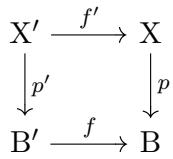
\includegraphics[keepaspectratio]{images/part001_48571453.jpg}}

是笛卡尔的。

映射 \(f\) 、\(f'\) 与 \(p'\) 都是连续的。方块 \((10')\) 的交换性由其定义得出。设 \(h_i\) 表示从 \(\mathrm{X}_i'\) 到 \(\mathrm{B}_i' \times_{\mathrm{B}} \mathrm{X}\) 上的典型同胚 (I, p. 8, 命题 2)，并设 \(h: \mathrm{X}' \to \mathrm{B}' \times_{\mathrm{B}} \mathrm{X}\) 为典型映射 (loc. cit.)。我们有 \(h = h'' \circ h'\) ，其中 \(h': \mathrm{X}' \to \coprod (\mathrm{B}_i' \times_{\mathrm{B}} \mathrm{X})\) 是由诸 \(h_i\) 诱导的同胚，而 \(h'': \coprod (\mathrm{B}_i' \times_{\mathrm{B}} \mathrm{X}) \to (\coprod \mathrm{B}_i') \times_{\mathrm{B}} \mathrm{X}\) 是在 I, p. 4 的例 5 中定义的那个映射。由 I, p. 8 的命题 2 即得结论。

例 2. --- 设 \((X,p)\) 为一个 B-空间，\((\mathrm{A}_{k})_{k\in\mathrm{K}}\) 为 B 的一族子空间。设 A 为族 \((\mathrm{A}_{k})_{k\in\mathrm{K}}\) 的和空间，Y 为族 \((\overline{p}^{1}(\mathrm{A}_{k}))_{k\in\mathrm{K}}\) 的和空间；用 \(i: A \to B\) 、\(j: Y \to X\) 与 \(p': Y \to A\) 分别表示由 \(A_{k}\) 到 B 中的典型单射、\(\overline{p}^{1}(\mathrm{A}_{k})\) 到 X 中的典型单射以及诸映射 \(p_{\mathrm{A}_{k}}: \overline{p}^{1}(\mathrm{A}_{k}) \to \mathrm{A}_{k}\) （\(k \in K\) ）所诱导的映射。方块

\[
\begin{array}{c} \mathrm{Y} \xrightarrow {j} \mathrm{X} \\ \Biggl \downarrow p ^ {\prime} \\ \mathrm{A} \xrightarrow {i} \mathrm{B} \end{array}\tag{11}
\]

是笛卡尔的；这由 I, p. 10 的例与命题 6 得出。

